\section{Auswahl der Komponenten}

Da beinahe keine Komponenten zugekauft werden mussten, und bei einigen Zukaufteilen keine Auswahl möglich war, musste nur bei drei Komponenten eine Entscheidung getroffen werden.
Allgemein spielten bei Wahl der Komponenten Preis und Lieferdatum die größte Rolle.
Dies rührt daher, dass beinahe in allen Fällen Modifikationen geplant waren, um eine bessere Integration in den Arbeitsbereich zu erreichen.

\subsection{Labor Spannungsversorgung}

Hier wurde das billigste Modell gewählt, welches alle Vorraussetzungen in ausreichendem Rahmen erfüllte.
Es handelt sich um eine Spannungsversorgung mit einem Funktionsbereich bis etwa 300 Watt (30 Volt und 10 Ampere), was für die vorliegenden Experimente als ausreichend erachtet wurde.

\begin{figure}[H]
    \begin{center}
        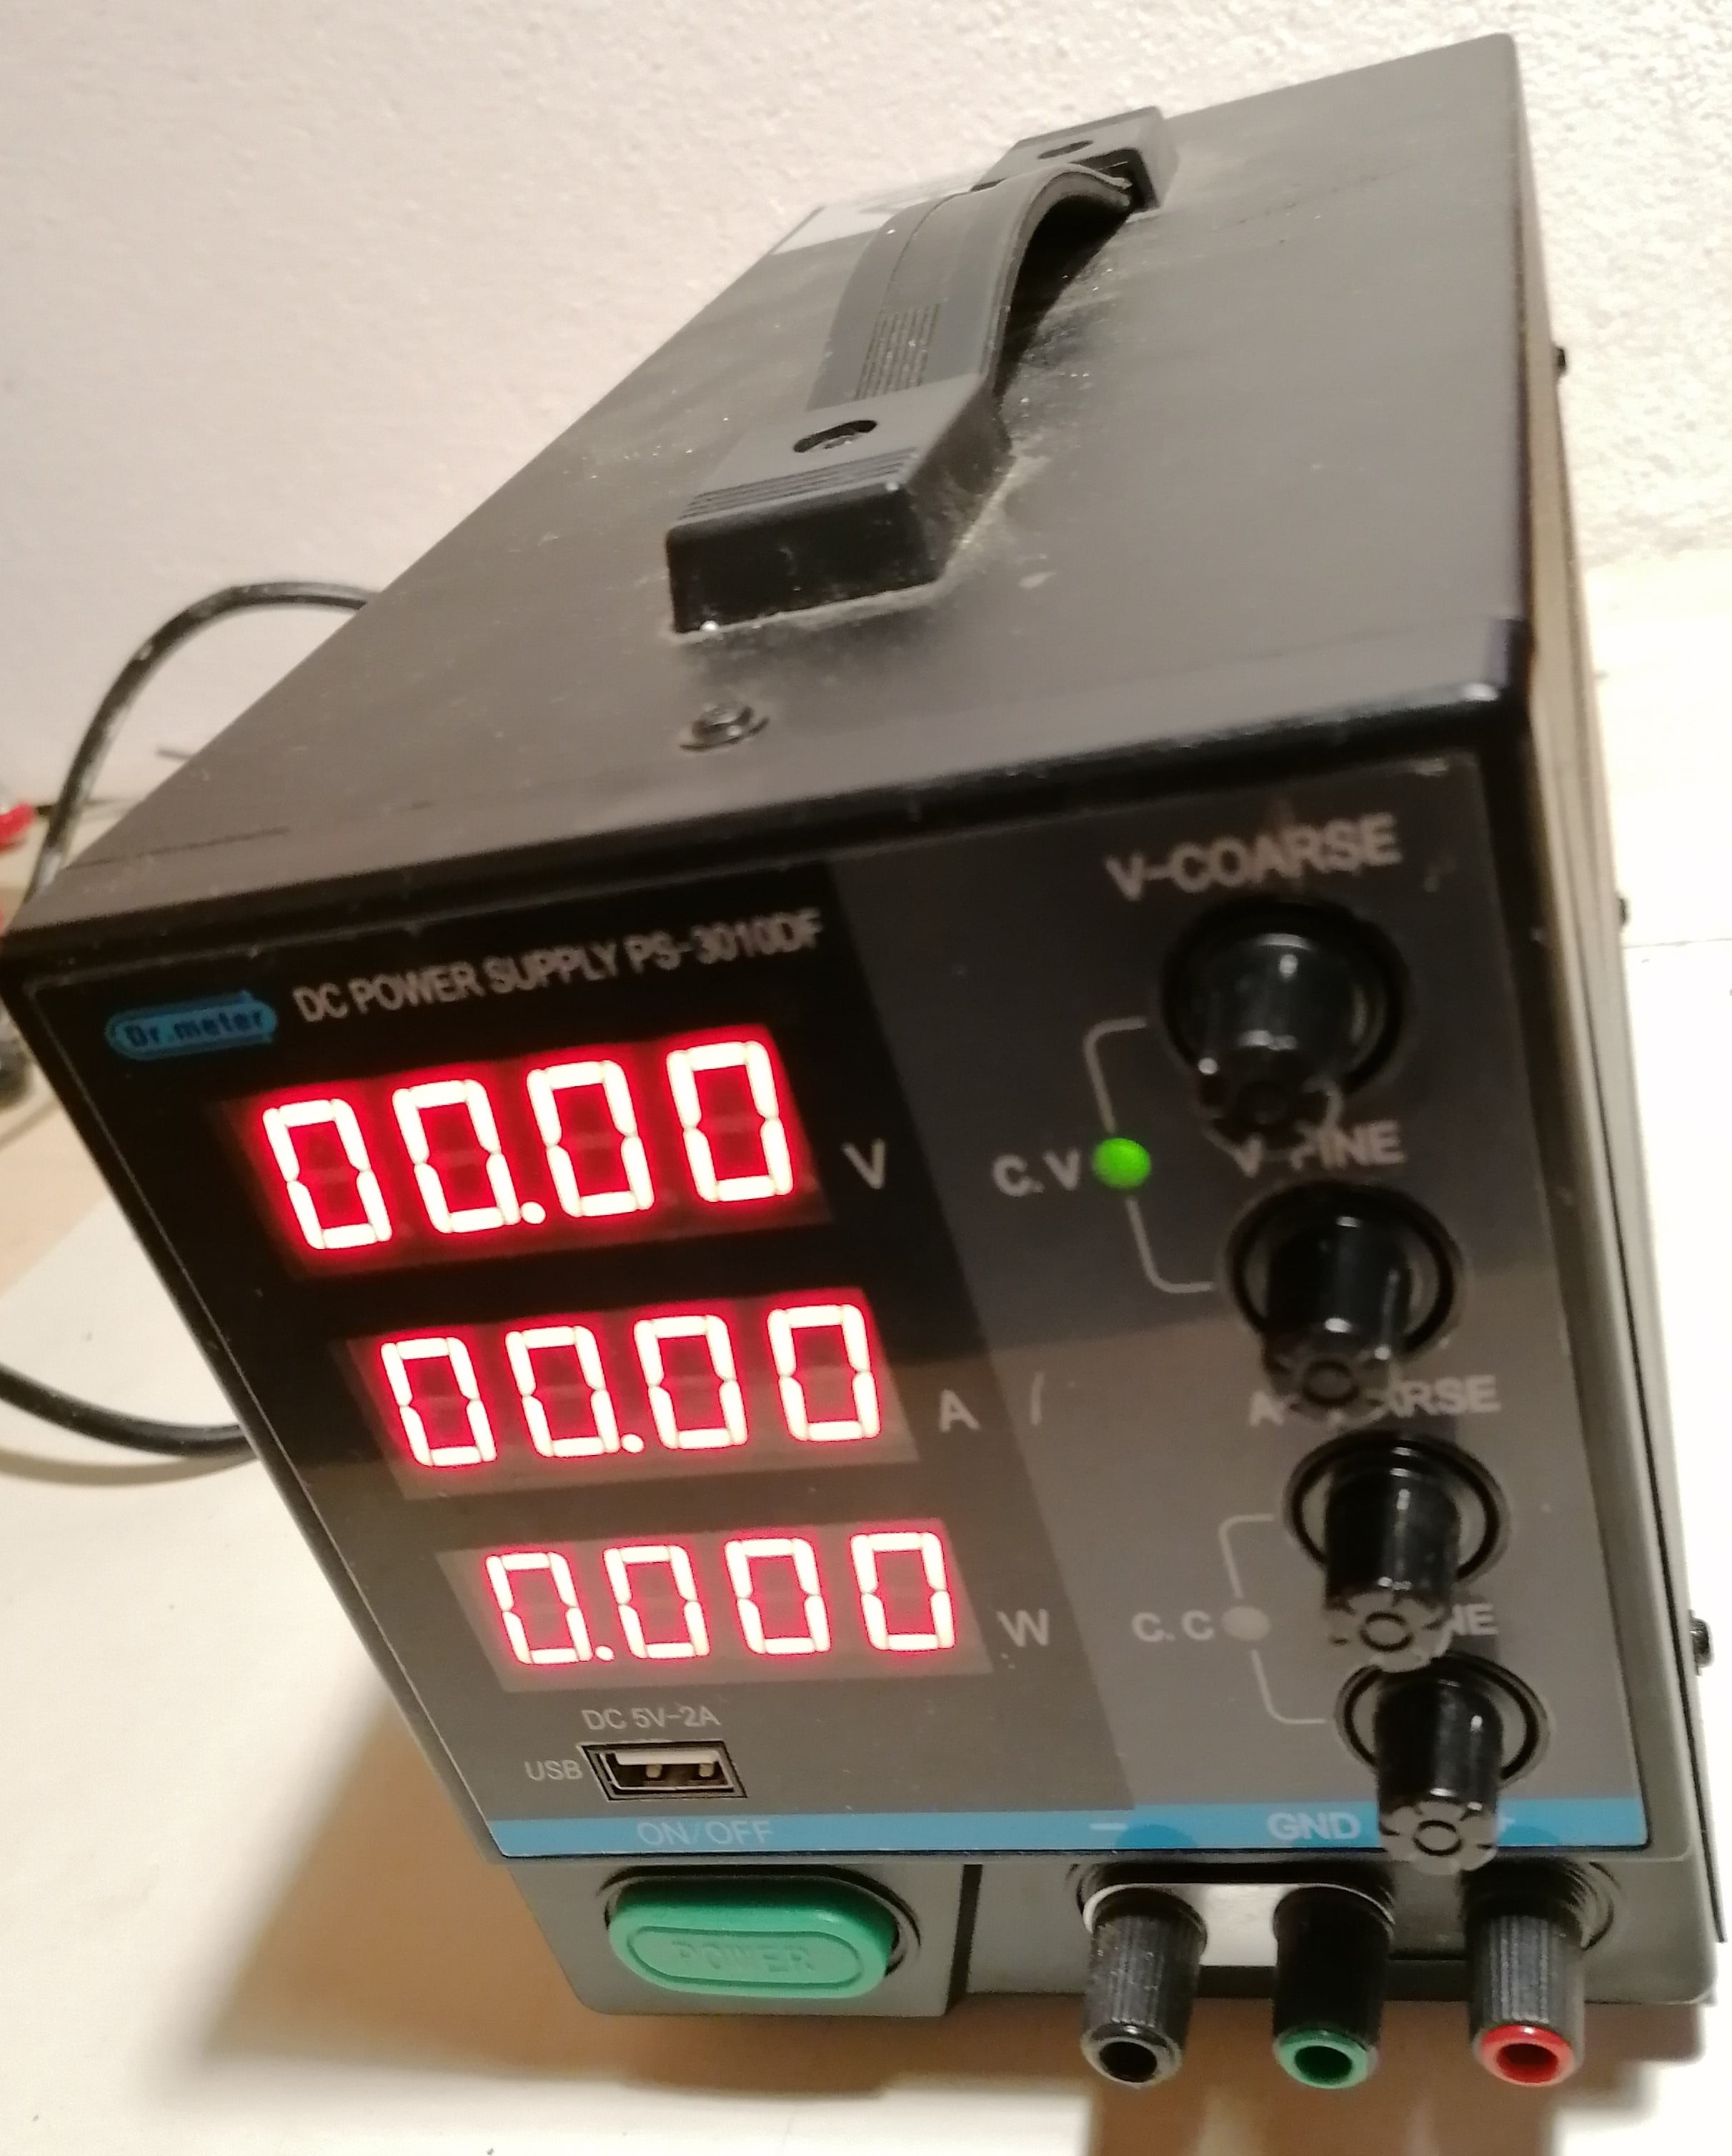
\includegraphics[width=0.3\textwidth]{spannungsversorgung.jpg}
        \caption{Die ausgewählte Labor Spannungsversorgung}
    \end{center}
\end{figure}

\subsection{Lötkolben}

Hier waren eine austauschbare Spitze, sowie einstellbare Temperatur die gewünschten Eigenschaften.
Die Entscheidung fiel auf ein Modell mit verstellbarer Temperatur zwischen 180 und 300 °C sowie zugehörigen Ersatzspitzen.

\begin{figure}[H]
    \begin{center}
        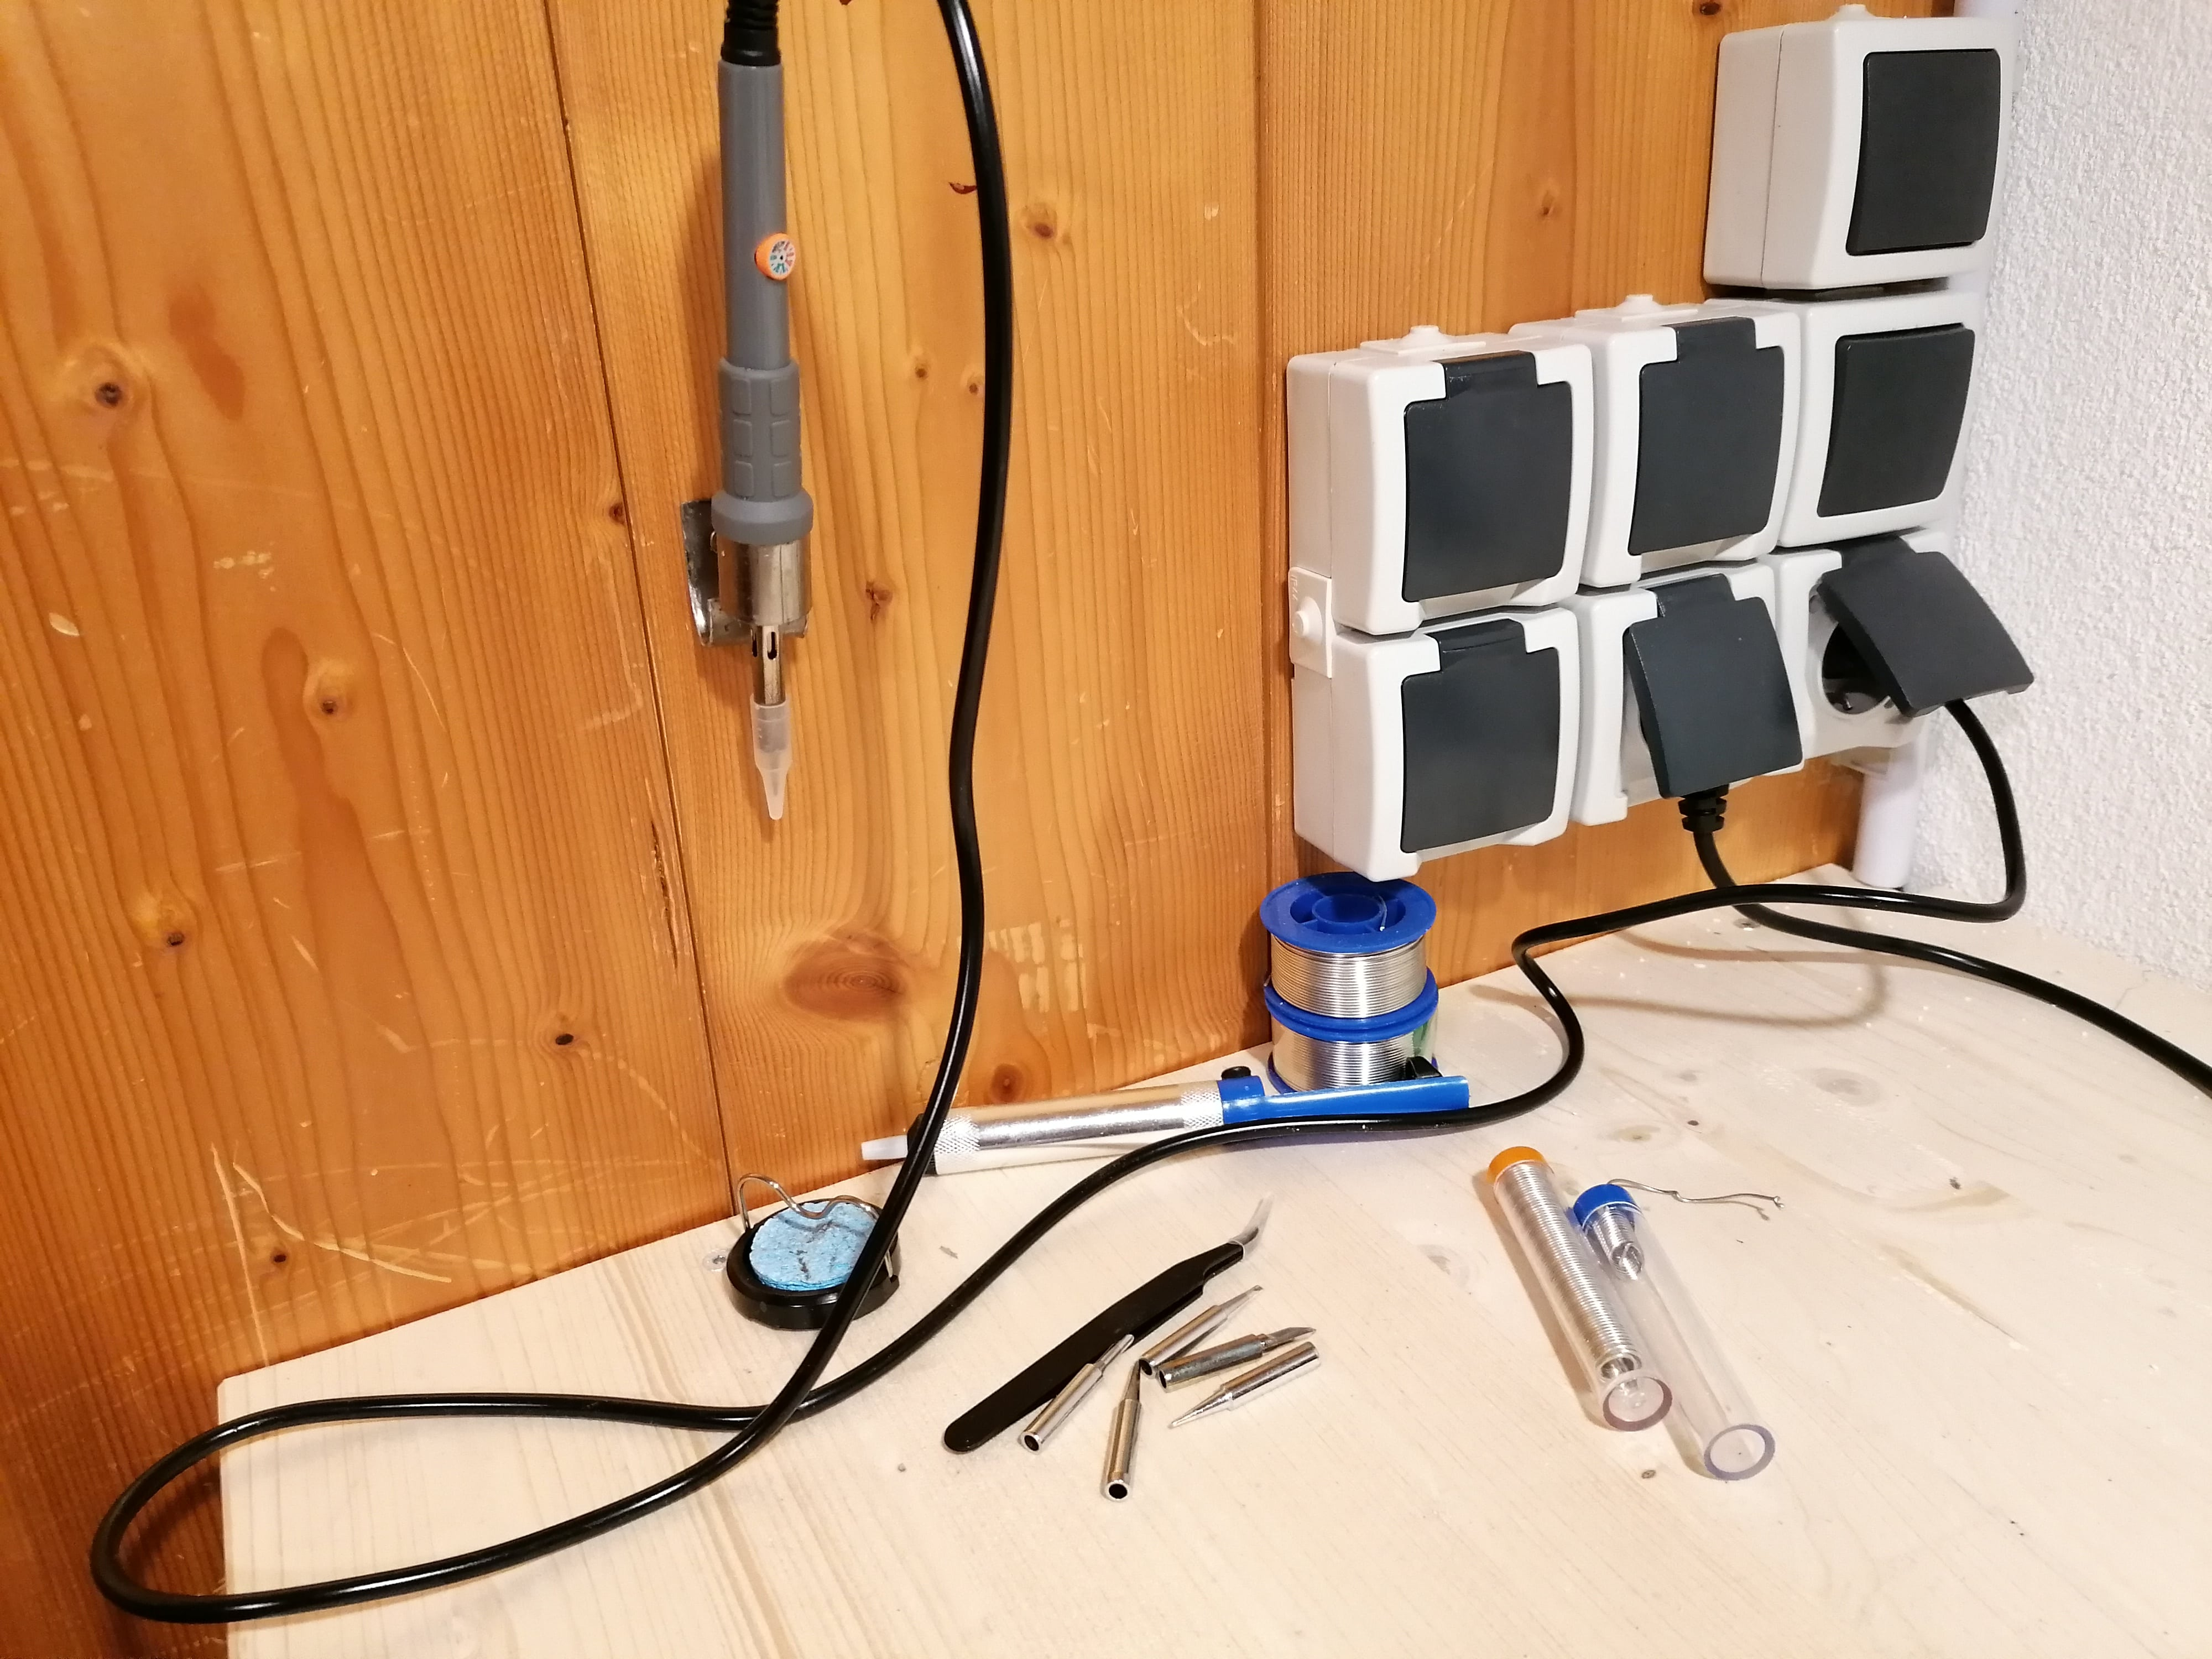
\includegraphics[width=0.3\textwidth]{loetkolben.jpg}
        \caption{Lötkolben mit Zubehör}
    \end{center}
\end{figure}

\subsection{Beleuchtung}

Bei Wahl der Beleuchtung spielte vor allem die Beweglichkeit des Leuchtkopfes eine Rolle. 
Weiters musste diese geignet sein um mit 230 Volt betrieben zu werden, da anstatt eines Steckers eine direkte geschaltene Verbindung zum Stromnetz geplant war.
Als Leuchtmittel wird eine 1600 Lumen LED-Glühbirne verwendet, um eine adäquate Beleuchtung zu erreichen.

\begin{figure}[H]
    \begin{center}
        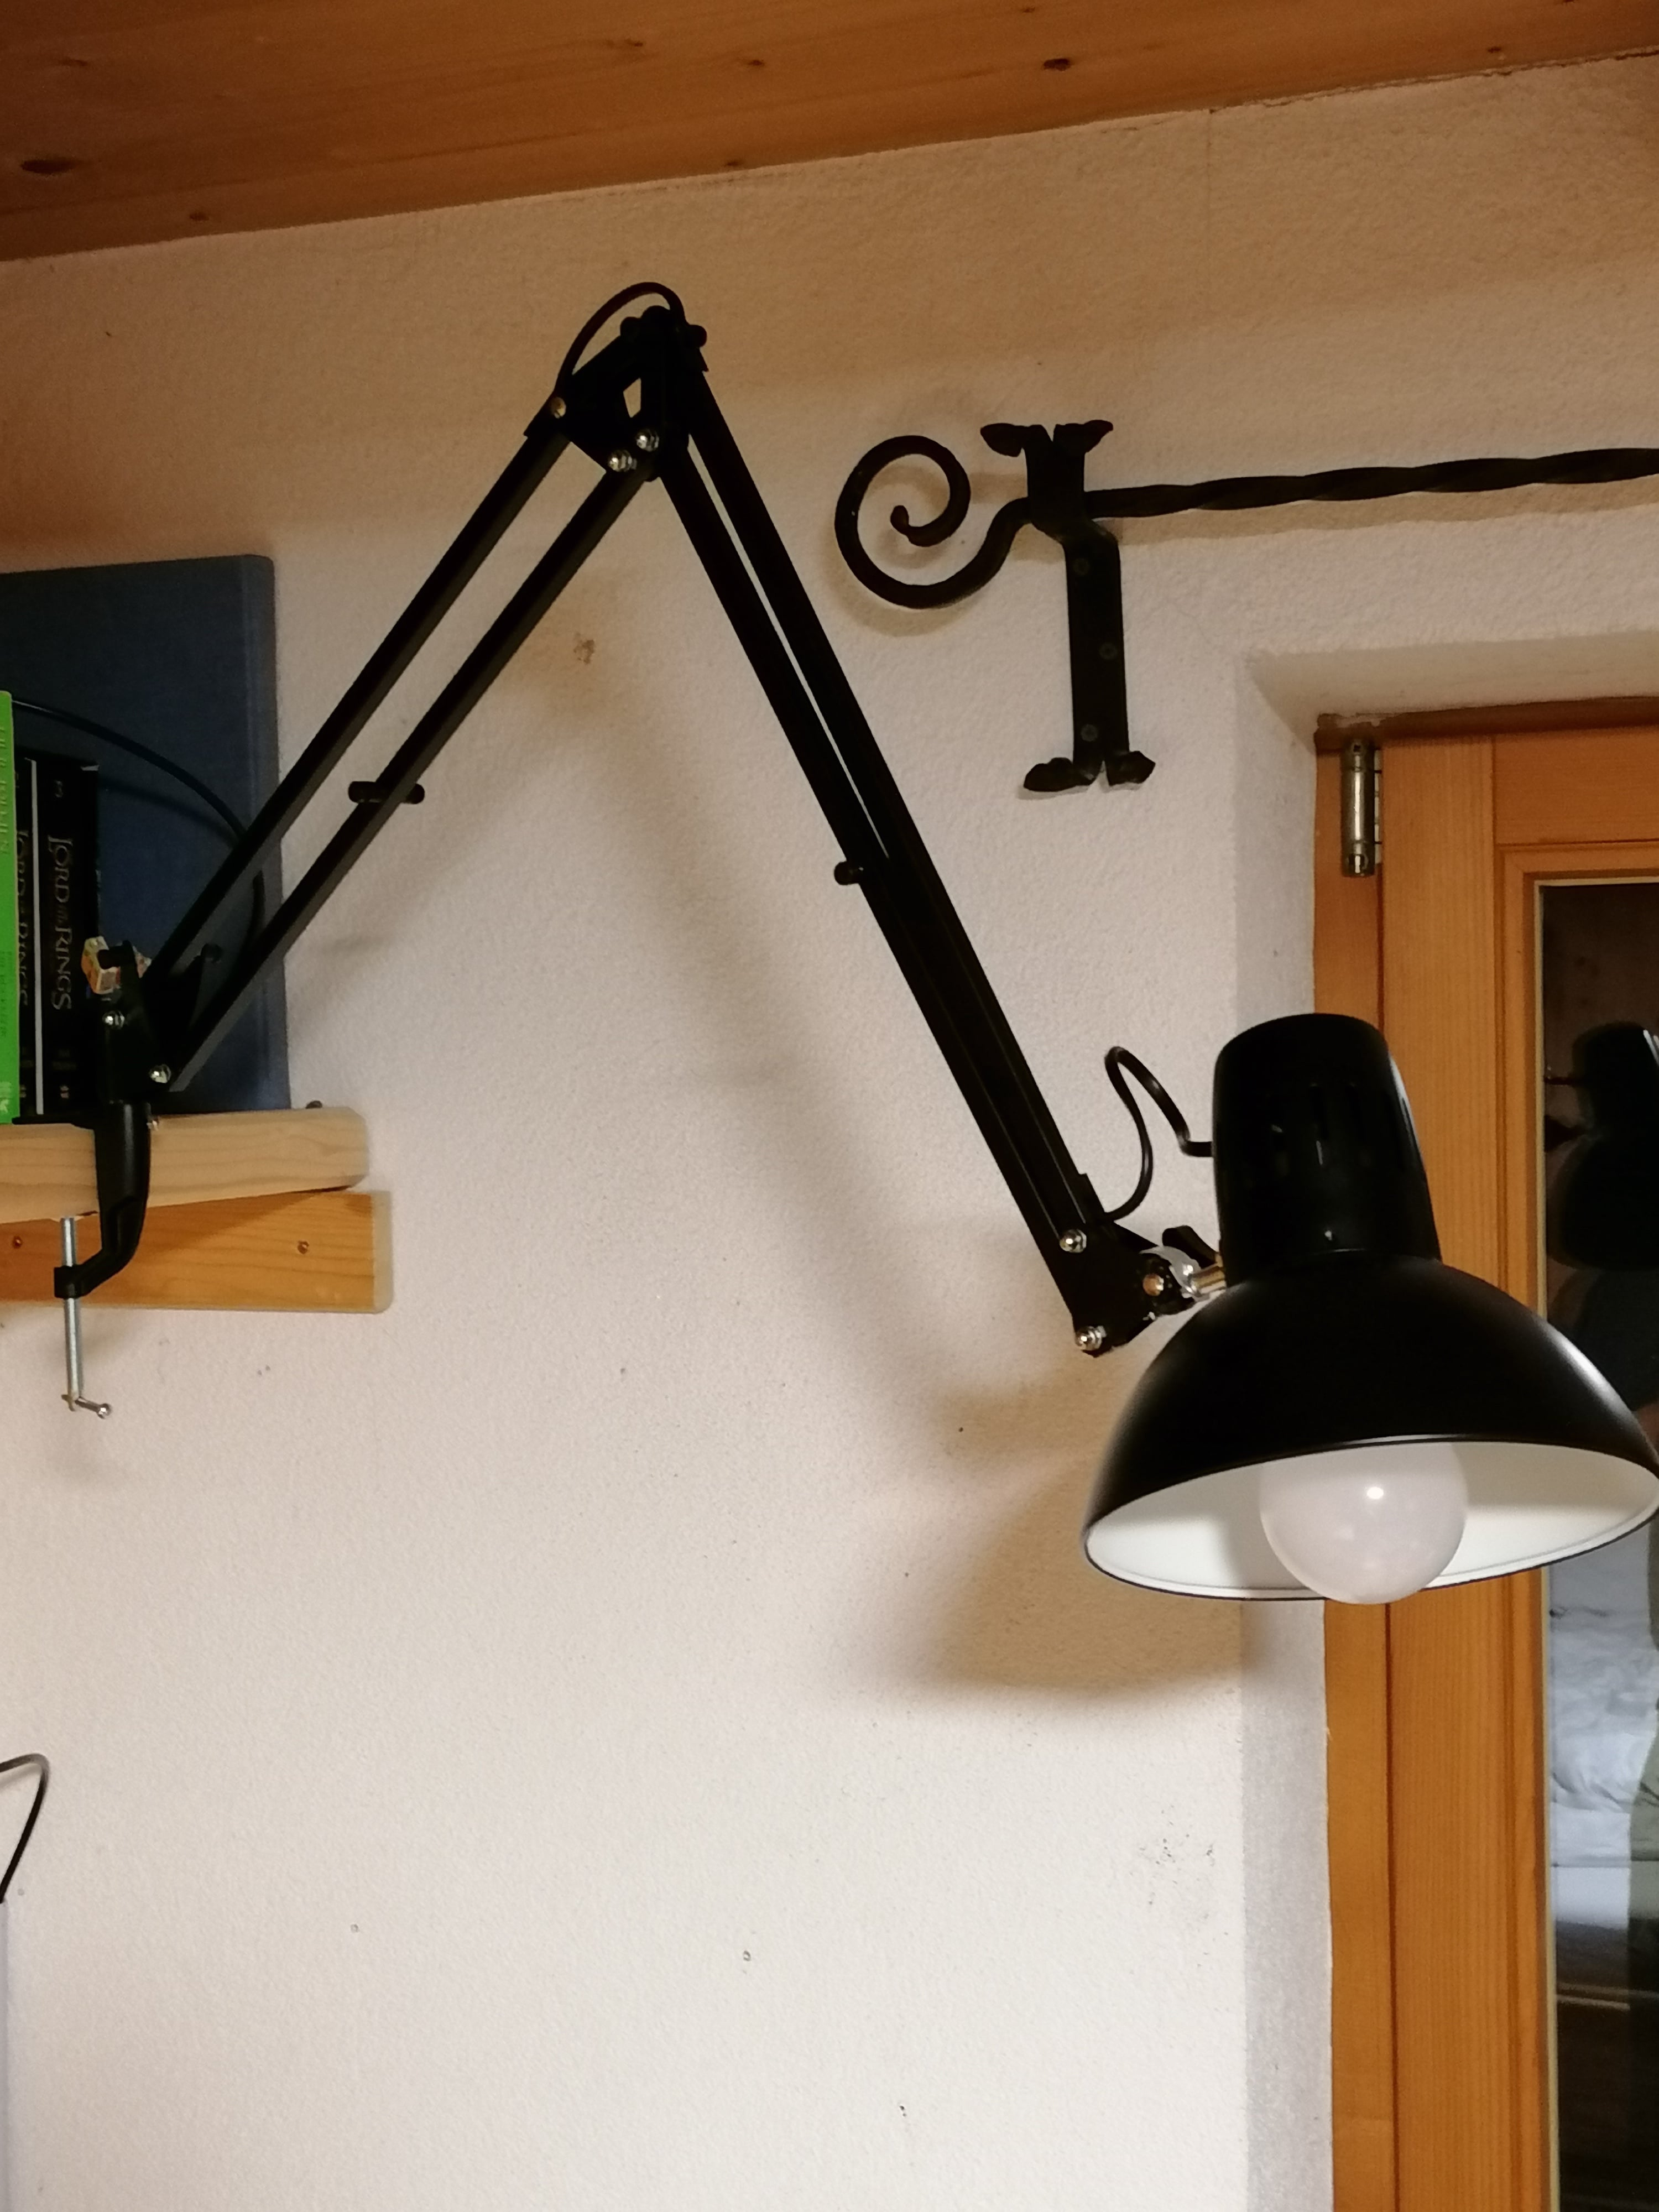
\includegraphics[width=0.3\textwidth]{lampe.jpg}
        \caption{Lampe montiert und angeschlossen}
    \end{center}
\end{figure}